\subsection{Character segmentation}
\label{sec:charseg}
Before we can feed the separate characters to our character classifiers, the word crops are processed by a character segmentation algorithm. First, the word crop images are binarized using the Otsu binarization method \cite{otsu1975threshold}. Then a histogram is created that contains the column-wise maximum consecutive number of white pixels. This histogram has local maximums at the points where there is a transition between two characters. In order to deal with the effect of noisy images, we apply an average smoothing with a window width of 5. Finally, we select the local maximums as possible cutting positions. An illustration can be found in Figure \ref{fig:char_seg}.

\begin{figure}
 \centering
 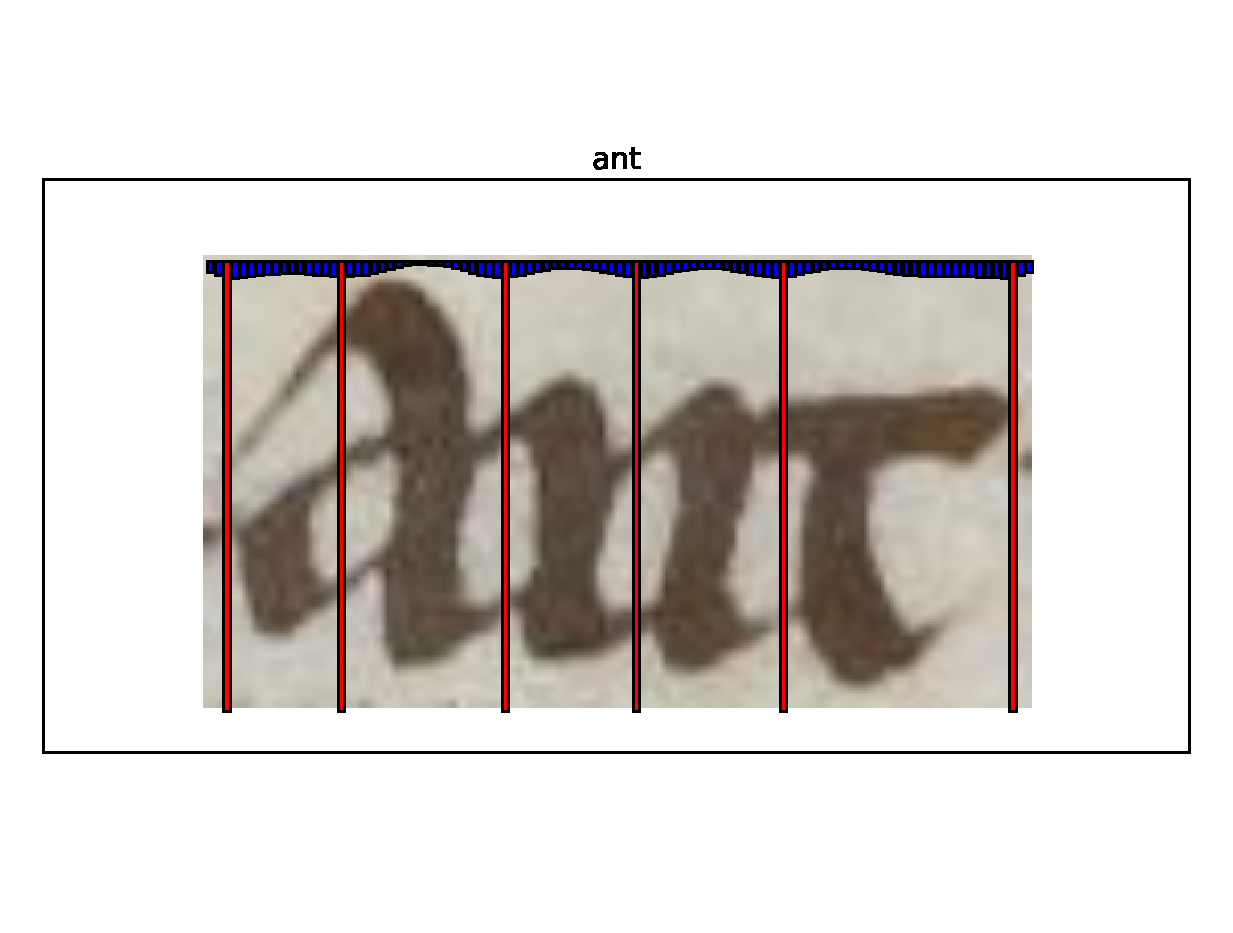
\includegraphics[width=.5\textwidth,trim={3cm 3cm 3cm 3cm},clip]{figures/char_segmentation.eps}
 \caption{Illustration of our character segmentation algorithm. It can be seen that the characters themselves are separated by the red lines. However, the \textit{a} and \textit{n} are also cut inside. At these points there clearly is a local maximum of consecutive white pixels.}
 \label{fig:char_seg}
\end{figure}

We restrict a single letter to be between 10 and 60 pixels wide. All other possible segmentations are ignored. We found that this method is somewhat greedy in the sense that there are a lot of false positives among the selected cutting positions. However, this was not considered harmful, since most invalid crops will lead to candidate words that are not plausible based on our vocabulary. The possible crops are first classified separately after which their predictions are combined to form words.